\section{Reweighting Method}
\label{sec:reweighting}

Monte Carlo simulations of physics processes are very heavily controlled in ATLAS. Each theoretical distribution must be validated, propagated through a detailed simulation of the ATLAS detector and unfolded through an digital approximation of instrumentation effects and reconstructed back in to physics objects in the same manner as the data. This leads to the production of MC samples being extremely costly in terms of computing resources.

Each sample produced is filtered by quark flavour and sliced in terms of the associated Boson Pt such the statistical accuracy of the samples can be enhanced. This means for a single physics process there is usually upwards of 20 samples required. If each generator variation would be simulated, more than 100 samples per process would be needed which is considered computationally impractical. 

Truth level samples were used to produce a 2 dimensional parametrisation of the variations [ref SUSY tool note] This allows the assessment of generator effects on differential distributions whilst only requiring a single file containing the parametrised weights. 

Preliminary investigations were performed by producing weights based on a 1-dimensional parameterisation  based  on  either pT(Z) or njets. For  the  case  where pT(Z)  was used  for  the  parameterisation process, poor modelling is found for the properties related to the jets (HT,pT(j1)etc),whilst using the jet multiplicity as the basis for the parameterisation leads to poor modelling ofthe ETmiss.  Due to this a 2D parameterisation was performed using both pT(Z) and njets. [ref SUSY tool note] given the goal of using this tool to assess variations in the Z$\rightarrow\tau\tau$ process, instead of pT(Z) the Visible Mass (mvis) was considered. This is a value more commonly used in cases where tau neutrinos are liable to produce a truth contribution to Et miss and therefore offset the reconstructed mass of the parent boson.

To cohere with the prior studies and to coincide with the Pt(Z) slicing of the samples the mvis paraemetrisation is produced in bins of [0,70], [70-140], [280-500], [500-700], [700-100], [1000-2000], [2000-ECMS] GeV and the jet multiplicity is binned in terms of 0,1,2,>2 jets. This averages out large differences that may occur in extremely high jet multiplicity regions (that this analysis is blind to) and allows for low statistical error in every bin.

For a given mvis bin (i), and njets bin (j), the weights are calculated per sample (up and down variations are treated separately) using:
\[W_{i,j}=
\frac{N_{i,j}^{Syst}}{N_{i,j}^{Nominal}}W_{i,j}
= \frac{\sum_{m_{\mathrm{T},flavour}}\sigma^{Syst}\cdot k\cdot\epsilon\cdot N_{i,j}^{Syst,RawNo}}{\sum_{p_{\mathrm{T},flavour}}\sigma^{Nominal}\cdot k\cdot\epsilon\cdot N_{i,j}^{Nominal,RawNo}}
\]

The largest variations expected are due to factorisation and renormalisation scales these can be seen in figure [\ref{fig:scales}] and the corresponding weights to be applied to the reconstructed nominal samples at truth level can be seen in figure [\ref{fig:weight}]

\begin{figure}[h!]
  \centering
   \subfloat[]{  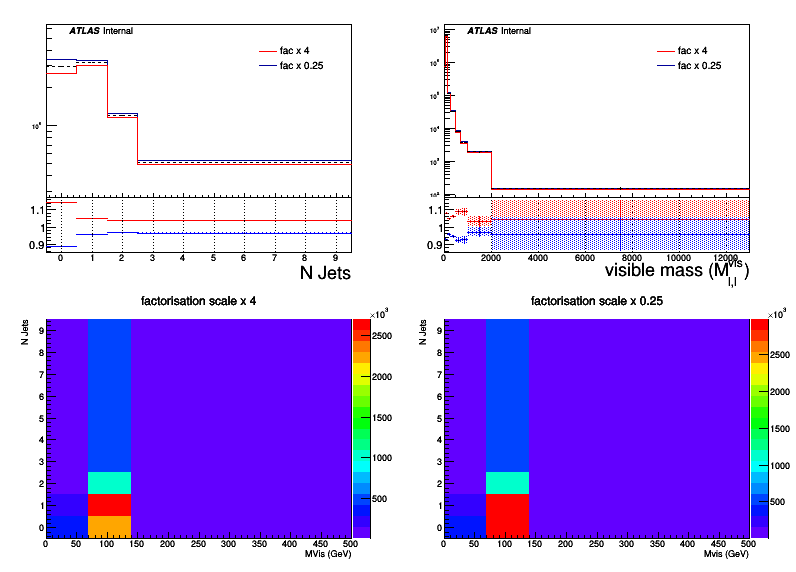
\includegraphics[width=\textwidth]{figures/fac}}

   \subfloat[]{  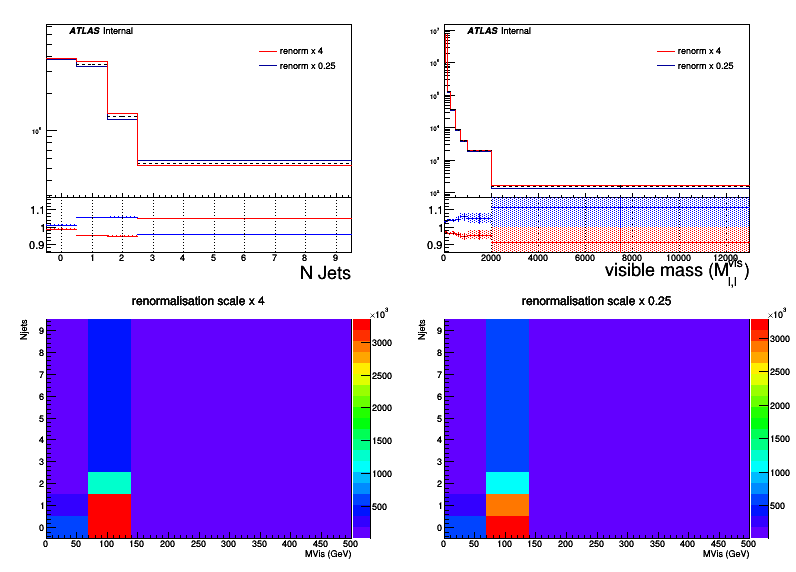
\includegraphics[width=\textwidth]{figures/ren}}
   \caption{Two dimensional parametrisation of variations due to changes in (a) factorisation and (b) renomalisation scale. The error can be taken as half the difference between up and down variations}
  \label{fig:scales}
\end{figure}

\begin{figure}[h!]
  \centering
   \subfloat[]{  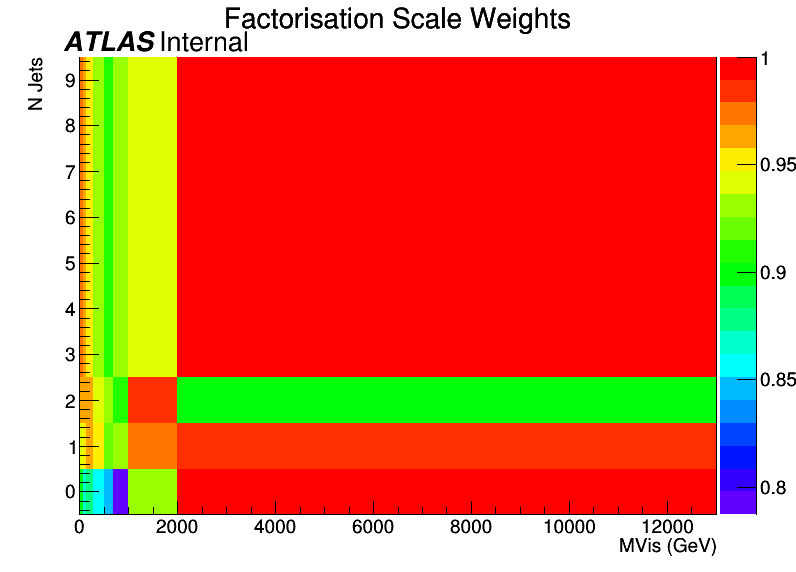
\includegraphics[width=0.7\textwidth]{figures/fac_weight}}

   \subfloat[]{  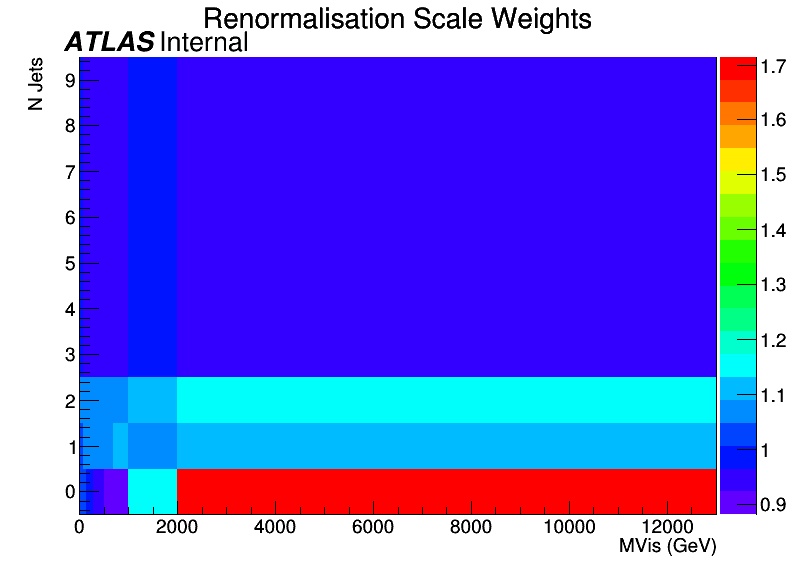
\includegraphics[width=0.7\textwidth]{figures/ren_weight}}
   \caption{Weights produced to emulate changes in (a)facorisation and (b) renomalisation scales. The weight should be positive for down variations and positive for up}
  \label{fig:weight}
\end{figure}

